\subsection{Drilling down the rabbit hole}
After login we are presented with a dashboard that shows a simple 
command line interface to ping the server. What we realize here is 
that chaining commands is possible if we use the \texttt{;} character.
We now have user access to the server. 
First test was to check if we could list the directory contents of 
the server:
\begin{figure}[htbp]
  \centering
  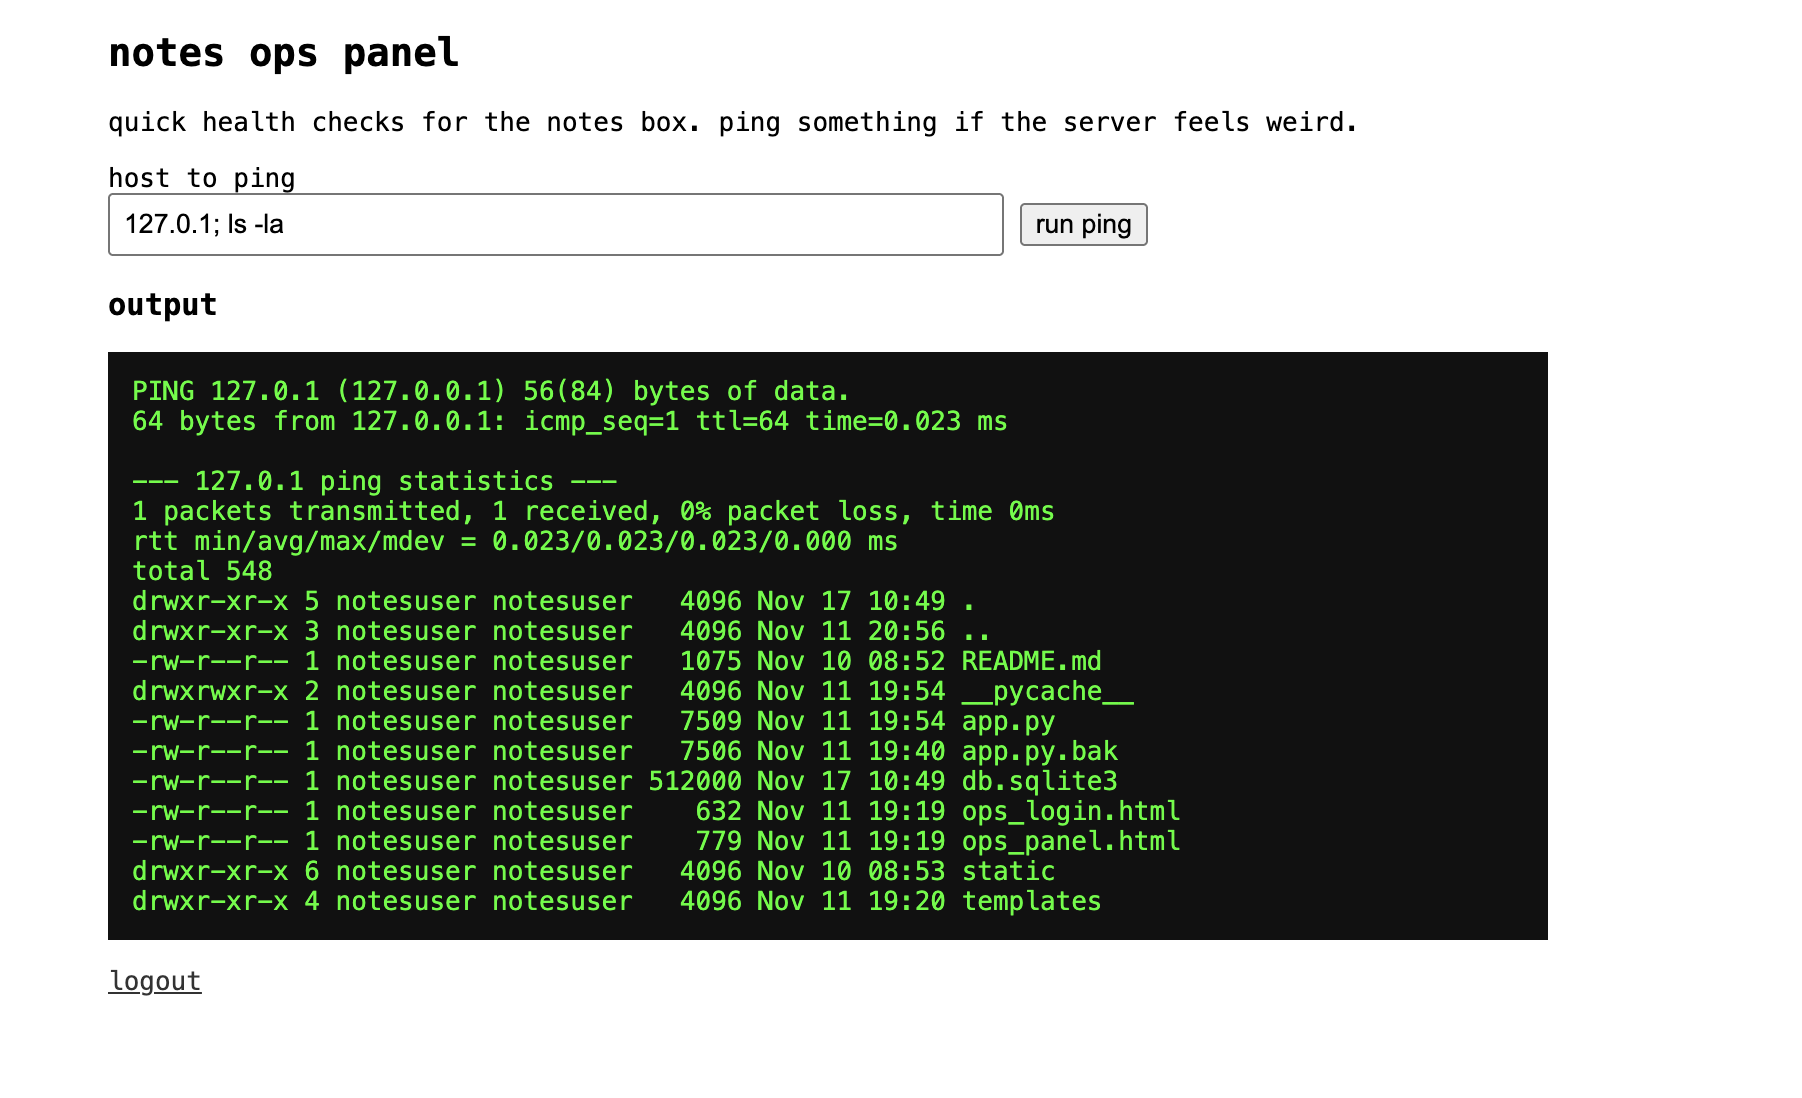
\includegraphics[width=1\linewidth]{images/ls_la_example.png}
  \caption{Listing the directory contents of the server.}
  \label{fig:sample}
\end{figure}

With this knowledge our next step is escalation of privileges. We have shell access
